% Chapter 3

\chapter{Identifying Alleles Associated with Disease Status and Proviral Load} 
\label{Chapter3}
\lhead{Chapter 3. \emph{Identifying Alleles Associated with Disease Status and Proviral Load}}

\section{Introduction}

Jeffery \emph{et al.} \citep{Jeffery1999, Jeffery2000} demonstrated the protective effects of the MHC class I alleles A*02 and Cw*08 in terms of disease status and a reduced proviral load in asymptomatic carriers of HTLV-I. It was also shown that B*5401 is associated with a greater risk of HAM/TSP and with a higher proviral load in HAM/TSP patients. Added to this, results showing that class I heterozygosity is associated with significantly lower proviral loads \citep{Jeffery2000} would suggest that the protective effect of the HLA haplotype extends to a range of alleles.

Using the same Kagoshima database as previous studies \citep{Jeffery1999, Jeffery2000}, our initial task was to reanalyze this data in an attempt to broadly classify the HLA class I alleles contained within the cohort into `detrimental', `beneficial' and `undefined' groups, according to their associations with disease risk and proviral load. This design would increase the power of the next stage of our study - understanding the functional basis of these associations though analysis of the HLA class I alleles' HTLV-I epitopes.

Hence, the aim of this chapter was to analyze the HLA class I repertoire of the Kagoshima cohort in terms of its association with proviral load and disease risk, using classical and novel nonparametric statistical methods.

\section{Methods}\label{chapter3/methods}

\subsection{The Kagoshima Dataset}\label{chapter3/kagoshima}

All HAM/TSP and AC subjects for this study were of Japanese ethnic origin, and resided in Kagoshima prefecture (1988 population: 1.7 million), southern Kyushu, Japan, where the seroprevalence of HTLV-I infection in adults is approximately 10\% \cite{Osame1986, Nakagawa1995}. The estimated prevalence of HAM/TSP in the HTLV-I positive population is less than 1\% \cite{Kaplan1990}. For the purposes of this study, 230 cases of HAM/TSP were compared with 202 randomly selected HTLV-I seropositive asymptomatic blood donors (asymptomatic carriers - ACs) from the Kagoshima Red Cross Blood Transfusion Service. The diagnosis of HAM/TSP was made according to World Health Organisation (WHO) criteria \cite{Osame1990}.

\subsection{Disease Risk}

The Yates $\chi^{2}$ test has been used to test the relationship between disease risk and the presence of an allele. The test takes as its input a matrix (table \ref{tables/chapter_4/table_1}) and examines the null hypothesis that the observed frequency of alleles in each population (HAM/TSP and asymptomatic carriers) is the same as the expected frequency. The Yates correction applied in each case is used to prevent overestimation of statistical significance for small amounts of data. 

\begin{table}[htbp]
\centering
\begin{tabular}{lll}
 & \textbf{A$^+$} & \textbf{A$^-$} \\
\hline
\textbf{D} & a & b \\
\textbf{H} & c & d \\
\hline
\end{tabular}
\caption[The input matrix for the $\chi^{2}$ test]{The input matrix for the $\chi^{2}$ test, where D = disease, H = health, A$^+$ = positive for protective allele and A$^-$ = negative for protective allele.}
\label{tables/chapter_4/table_1}
\end{table}

\subsection{Proviral Load}\label{chapter3/methodsLoad}

We used the Mann-Whitney $U$ test to examine the null hypothesis that the presence of a single allele had any effect on proviral load. This analysis was performed separately for HAM/TSP patients and asymptomatic carriers (ACs) as there is a very strong association between HAM/TSP and high proviral load. 

A novel ranking test was also formulated to examine the robustness of each allele's association with proviral load. For both groups (HAM/TSP and ACs), the following was performed: 

\begin{itemize}
	\item The individuals in each group were randomly assigned to two separate populations.
	\item For each of the two populations, the alleles were ranked in terms of the median proviral load associated with that allele (i.e.~the median proviral load of all individuals who possessed that specific allele). This random assignment was reiterated 1,000 times. 
	\item The result of this was 2,000 rank positions for each allele in terms of median proviral load. 
	\item The median rank and confidence intervals were then compared. 
\end{itemize}

\section{Results}

\subsection{Proviral Load}\label{chapter3/ResultsLoad}

\fref{chapter3/figureLoad} shows the results of the initial analysis of multiple Mann-Whitney $U$ tests for each allele. 

\fref{chapter3/figureRobust} shows the results of the robustness of rank measure in terms of proviral load. Any allele showing a narrow confidence interval is demonstrating a robust rank in the face of random sampling from the proviral load associated with it. For example, in the HAM/TSP results, we can be confident in the designation of HLA-A*03 as a 'good allele' in terms of proviral load, owing to its position on the x-axis and the narrowness of the confidence interval. From this data, alleles were designated as positive or negative according to the non-overlapping of their confidence intervals (\tref{chapter3/tableSummary}).

\subsection{Disease Risk}\label{chapter3/ResultsRisk}

\fref{chapter3/figureChi} shows the alleles ranked in terms of disease risk. These results show an obvious overlap with previous research (the significant results of A*02, B*54 and Cw*08) and the possibility of other candidate alleles (B*48).

\begin{table}[htp]
\begin{center}
\begin{sideways}
{
\scriptsize
\begin{tabular}{|c|c|c|c|c|c|c|c|c|c|c|}
\hline
Names & $P$ HAM/TSP & HAM/TSP Effect & $P$ AC & AC Effect & $P\ \chi^2$ & $\chi^2$ Effect & HAM/TSP Rank & AC Rank \bigstrut \\
\hline
A01 & 0.0000 & NA & 0.1786 & protective & 0.0000 & NA & & protective \bigstrut[t] \\
A02 & 0.3003 & protective & 0.0161 & protective & $< 0.0001$ & protective & & \\
A03 & 0.1464 & protective & 0.7909 & protective & 0.5261 & protective & protective & \\
A11 & 0.3999 & protective & 0.9211 & protective & 0.3635 & detrimental & & \\
A24 & 0.4787 & detrimental & 0.3681 & detrimental & 0.1474 & detrimental & & \\
A26 & 0.5197 & protective & 0.0437 & detrimental & 0.8559 & detrimental & & detrimental \\
A30 & 0.0568 & protective & 0.0000 & NA & 0.0000 & NA & protective & \\
A31 & 0.7096 & detrimental & 0.9037 & protective & 0.2681 & detrimental & & \\
A32 & 0.2803 & protective & 0.1786 & protective & 0.5365 & protective & protective & protective \\
A33 & 0.1514 & detrimental & 0.3850 & protective & 0.2995 & detrimental & detrimental & \\
B07 & 0.0230 & protective & 0.0963 & detrimental & 0.1035 & detrimental & & \\
B13 & 0.7524 & protective & 0.5186 & detrimental & 0.4508 & detrimental & & \\
B15 & 0.2597 & protective & 0.2601 & protective & 0.1281 & protective & & \\
B27 & 0.5412 & detrimental & 0.4263 & protective & 0.8839 & protective & detrimental & \\
B35 & 0.1039 & protective & 0.4310 & detrimental & 0.5841 & protective & & \\
B37 & 0.0000 & NA & 0.1786 & protective & 0.0000 & NA & & protective \\
B38 & 0.1893 & protective & 0.0000 & NA & 0.0000 & NA & protective & \\
B39 & 0.3045 & detrimental & 0.7824 & detrimental & 0.6011 & protective & & \\
B40 & 0.4786 & detrimental & 0.5709 & protective & 0.1104 & protective & & \\
B41 & 0.0000 & NA & 0.7562 & detrimental & 0.0000 & NA & & detrimental \\
B44 & 0.2169 & protective & 0.0733 & protective & 0.4486 & protective & & \\
B46 & 0.9813 & detrimental & 0.7261 & protective & 0.4279 & protective & & \\
B48 & 0.7705 & protective & 0.4001 & protective & 0.0263 & protective & & \\
B51 & 0.3067 & detrimental & 0.7686 & detrimental & 0.3218 & detrimental & & \\
B52 & 0.6364 & detrimental & 0.3742 & detrimental & 0.5040 & protective & & \\
B54 & 0.0034 & detrimental & 0.8505 & detrimental & 0.0008 & detrimental & detrimental & \\
B55 & 0.6298 & detrimental & 0.3022 & protective & 0.5622 & detrimental & & \\
B56 & 0.1452 & detrimental & 0.4664 & protective & 0.7439 & detrimental & detrimental & \\
B57 & 0.0000 & NA & 0.7432 & detrimental & 0.0000 & NA & & detrimental \\
B58 & 0.3457 & detrimental & 0.8068 & detrimental & 0.3748 & detrimental & & \\
B59 & 0.9265 & detrimental & 0.9980 & protective & 0.5947 & protective & & \\
B67 & 0.9677 & protective & 0.6816 & detrimental & 0.8012 & protective & & \\
C01 & 0.0716 & detrimental & 0.2828 & protective & 0.1416 & detrimental & detrimental & \\
C03 & 0.1176 & protective & 0.4690 & detrimental & 0.1659 & protective & & \\
C04 & 0.7755 & detrimental & 0.4697 & detrimental & 0.8566 & detrimental & & \\
C05 & 0.2803 & protective & 0.0438 & protective & 0.5261 & protective & protective & protective \\
C06 & 0.0161 & protective & 0.1786 & protective & 0.7092 & detrimental & protective & protective \\
C07 & 0.3218 & protective & 0.1859 & detrimental & 0.2001 & detrimental & & detrimental \\
C08 & 0.2647 & protective & 0.0466 & protective & 0.0029 & protective & & \\
C12 & 0.8432 & protective & 0.6302 & detrimental & 0.9447 & protective & & \\
C14 & 0.2828 & detrimental & 0.9638 & protective & 0.2323 & detrimental & & \\
C15 & 0.0170 & protective & 0.9644 & detrimental & 0.1904 & protective & protective & \bigstrut[b] \\
\hline 
\end{tabular}
}
\end{sideways}
\end{center}
\caption[The summary of allele association statistics]{The summary of allele association statistics. The first 4 columns give the $P$ values and the direction of effect for the Mann-Whitney $U$ tests of proviral load in both HAM/TSP patients and ACs for alleles in the Kagoshima cohort (\fref{chapter3/figureLoad}). For each allele, the proviral load of individuals with and without the allele was compared. The next 2 columns show the significance and direction of disease risk associated with the allele in question (\fref{chapter3/figureChi}). The last 2 columns show the significant results of the robustness of rank measure (\fref{chapter3/figureRobust}). For both HAM/TSP patients and ACs, alleles are described as `positive' if their upper confidence limit does not overlap with the lower confidence limit of the `detrimental' alleles (and conversely for the detrimental alleles).}
\label{chapter3/tableSummary}
\end{table}

\begin{figure}[htp]
\centering
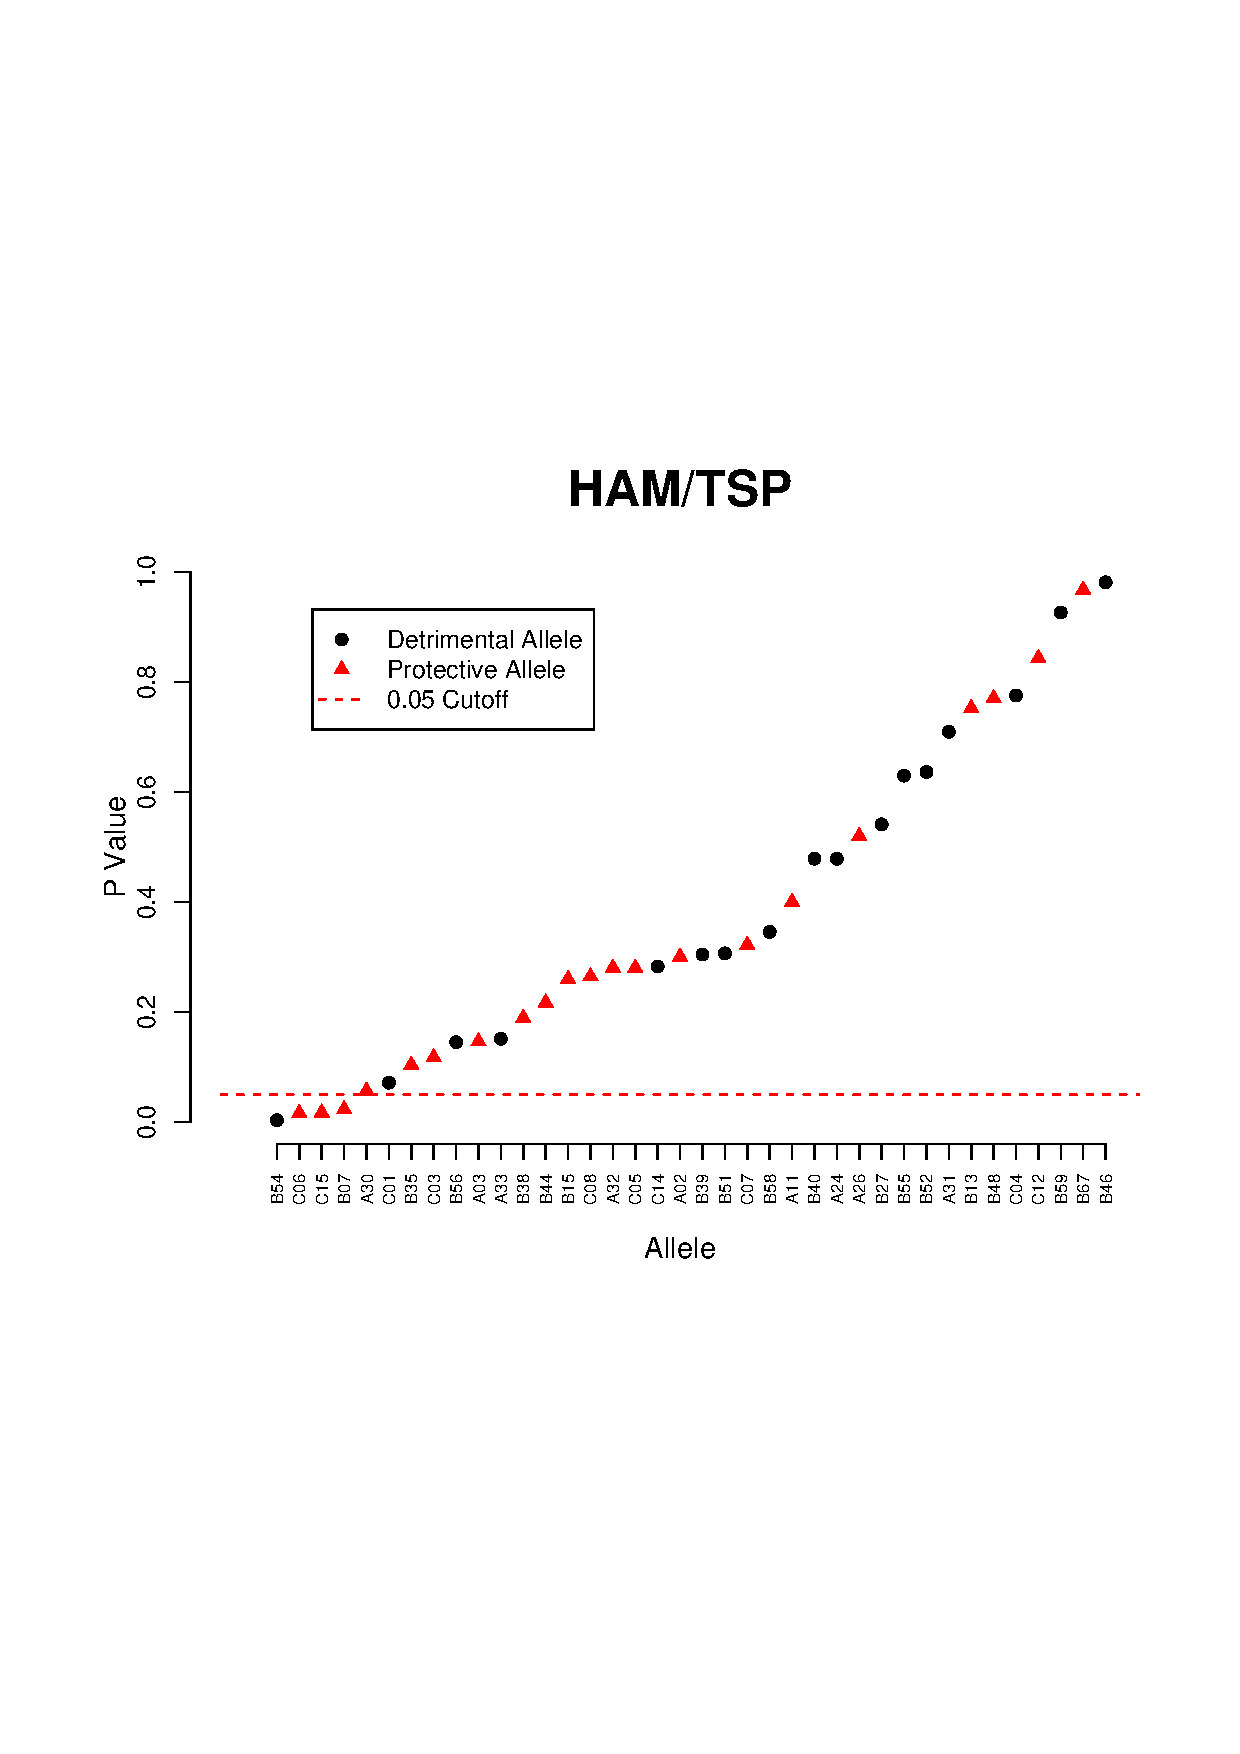
\includegraphics[width=14cm]{./Figures/chapter3/figureWilcoxHam} \\
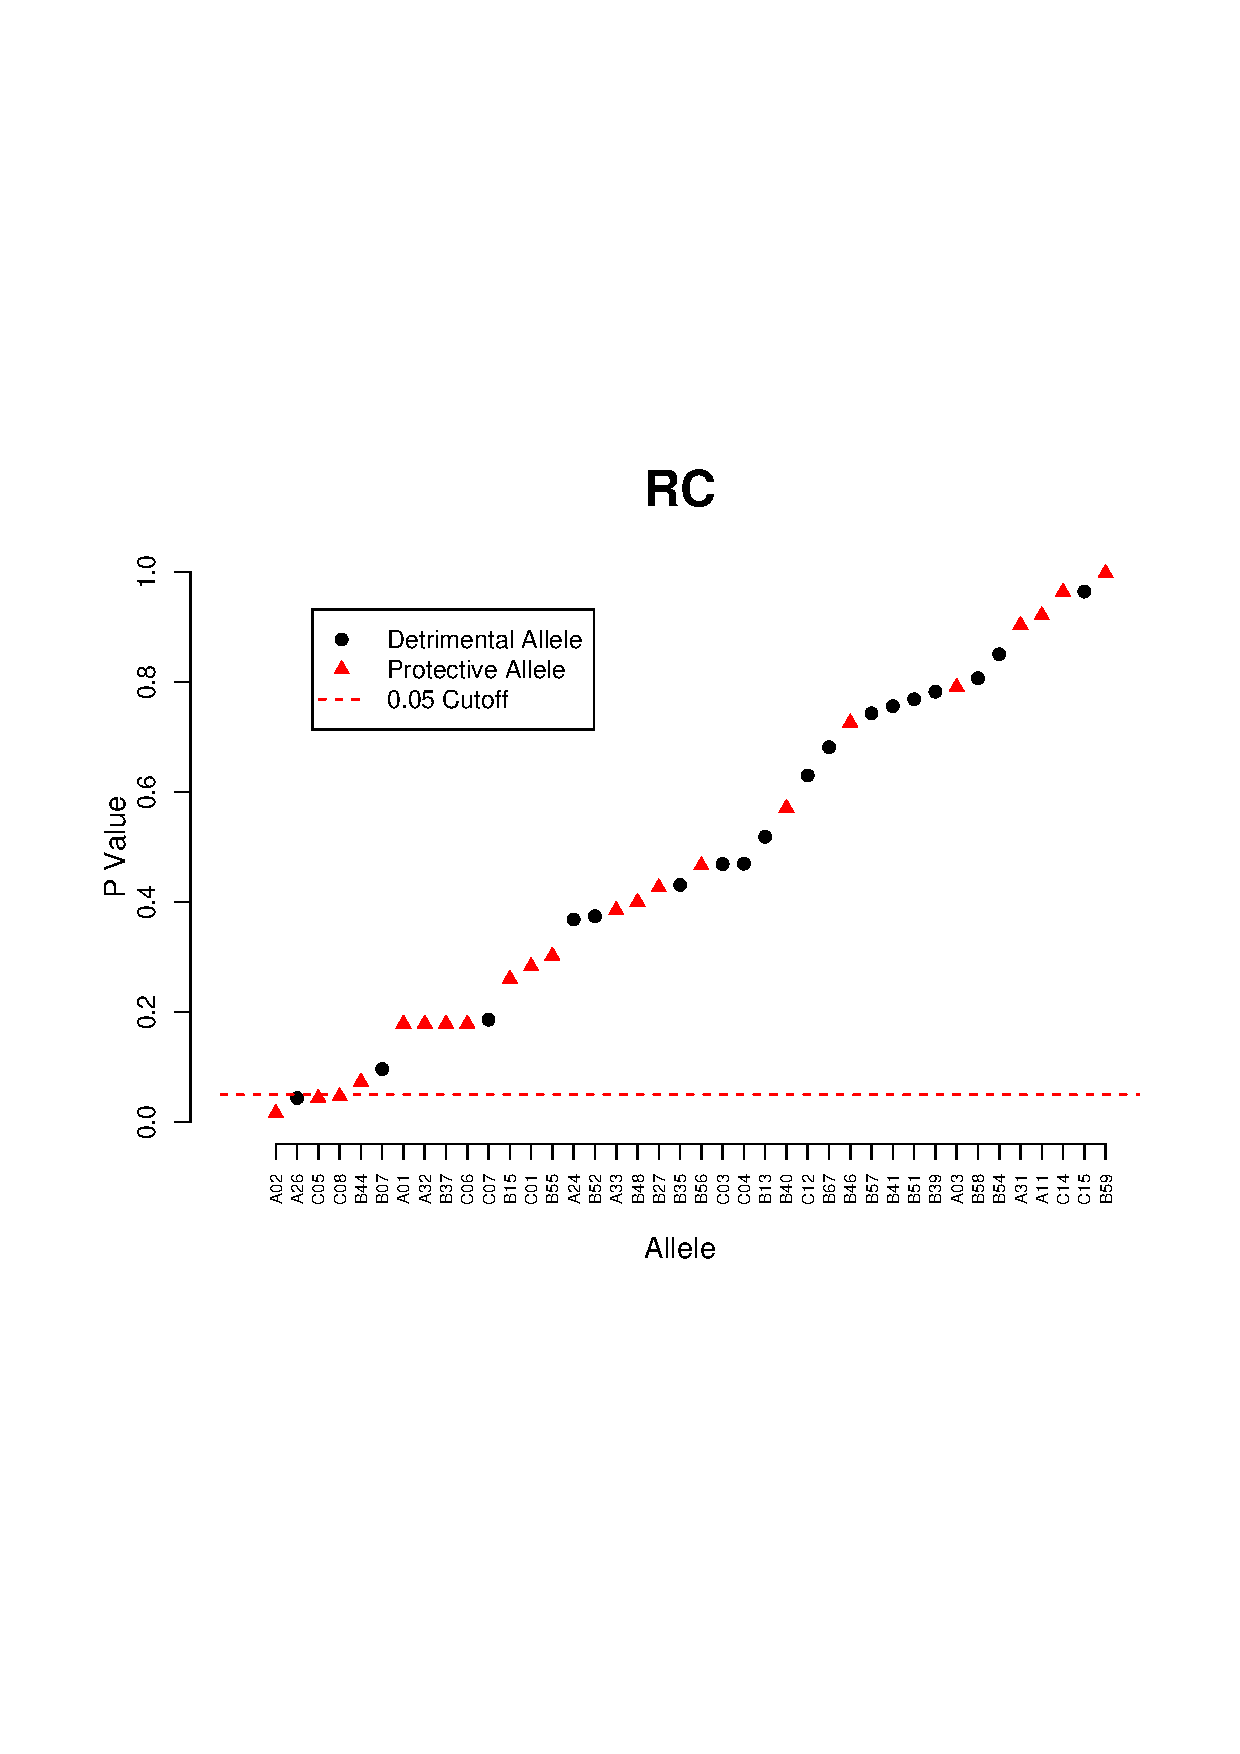
\includegraphics[width=14cm]{./Figures/chapter3/figureWilcoxAC}
\caption[Allele rankings for proviral load association]{The allele population of the HAM/TSP and AC individuals ranked by their Mann-Whitney $U$-test $P$ values, as described in \sref{chapter3/methodsLoad}. The black circle indicates that the association is negative (the presence of the allele is associated with a higher proviral load) and the red triangle indicates a positive association.}
\label{chapter3/figureLoad}
\end{figure}

\begin{figure}[htp]
\centering
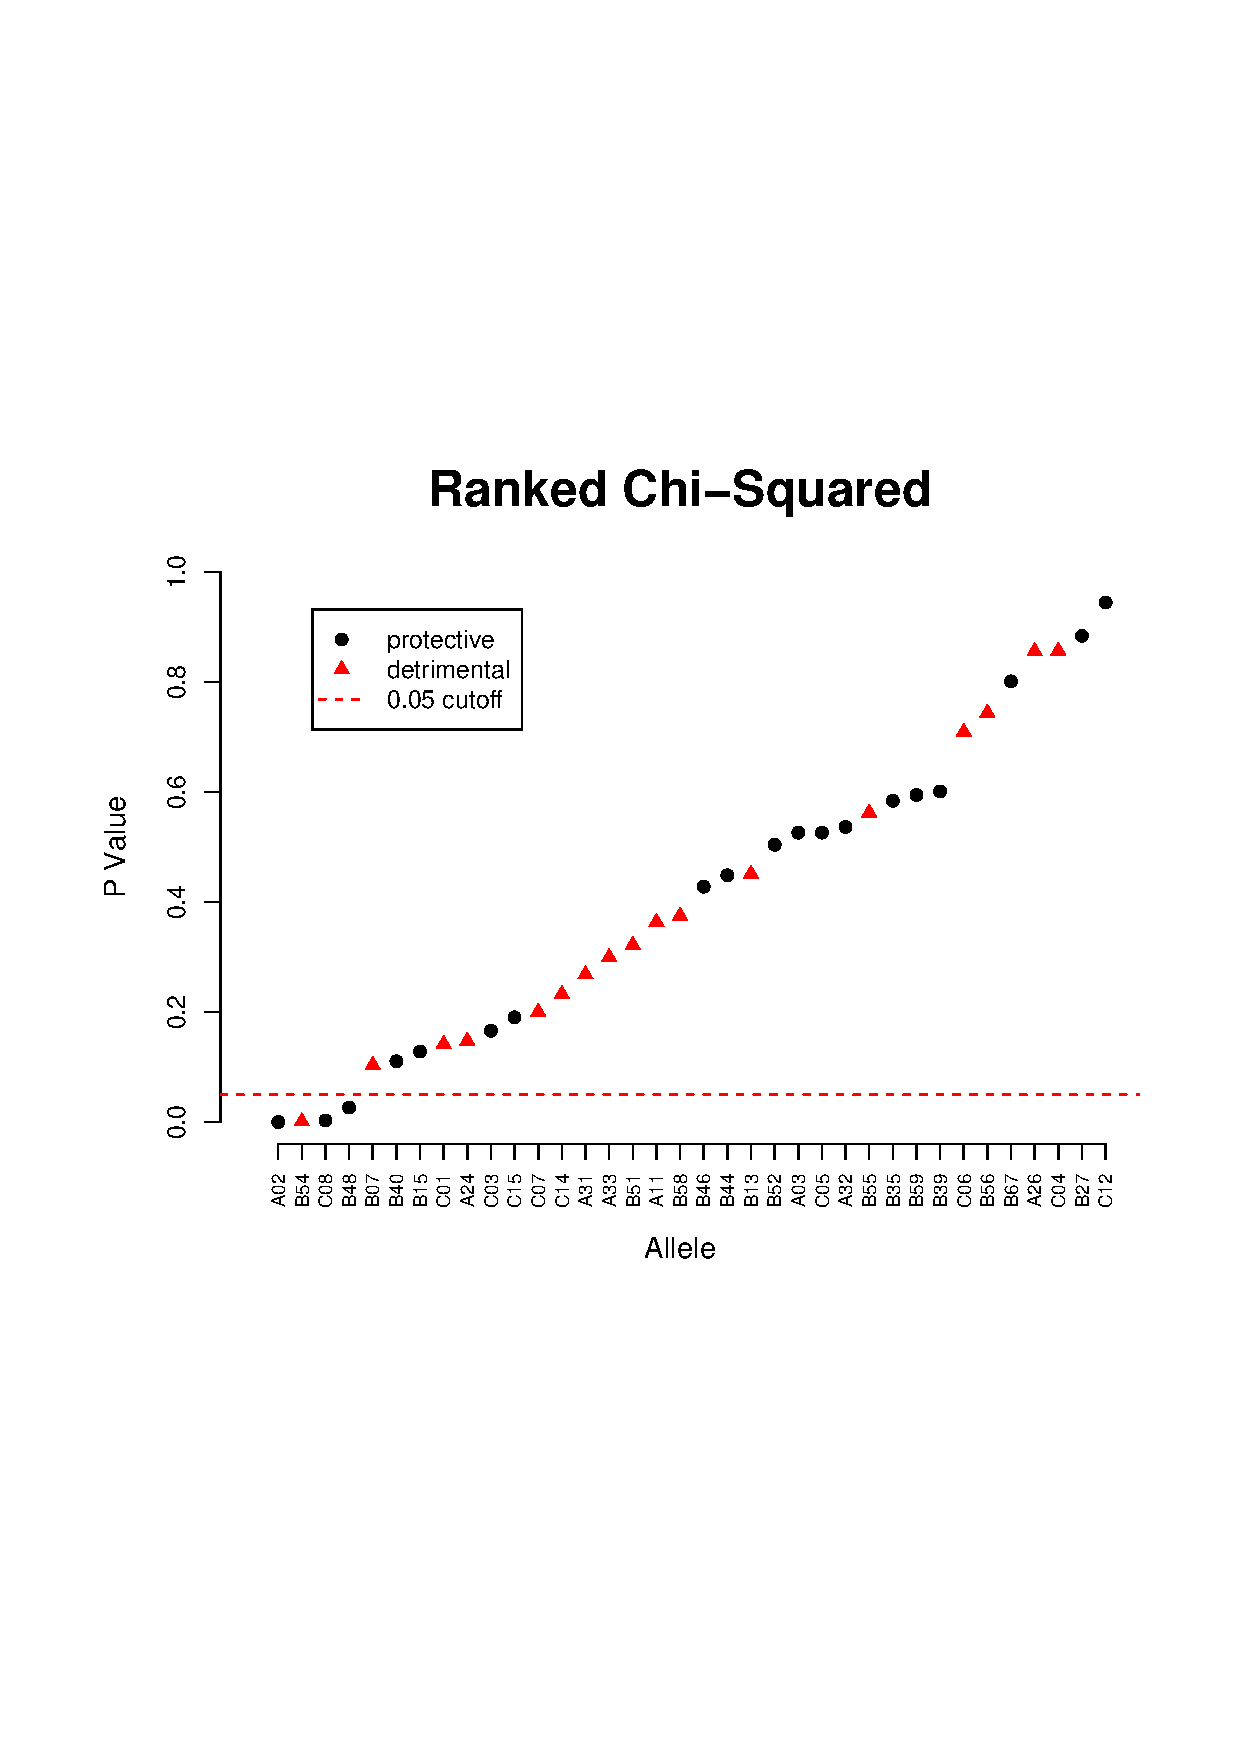
\includegraphics[width=14cm]{./Figures/chapter3/figureChi}
\caption[]{The result of the Yates $\chi^2$ analysis of disease risk for all alleles in the Kagoshima population. The black circles indicate a protective effect of an allele, the red trangle a detrimental effect. The red dotted line represents significance at $P = 0.05$.}
\label{chapter3/figureChi}
\end{figure}

\begin{figure}[htp]
\centering
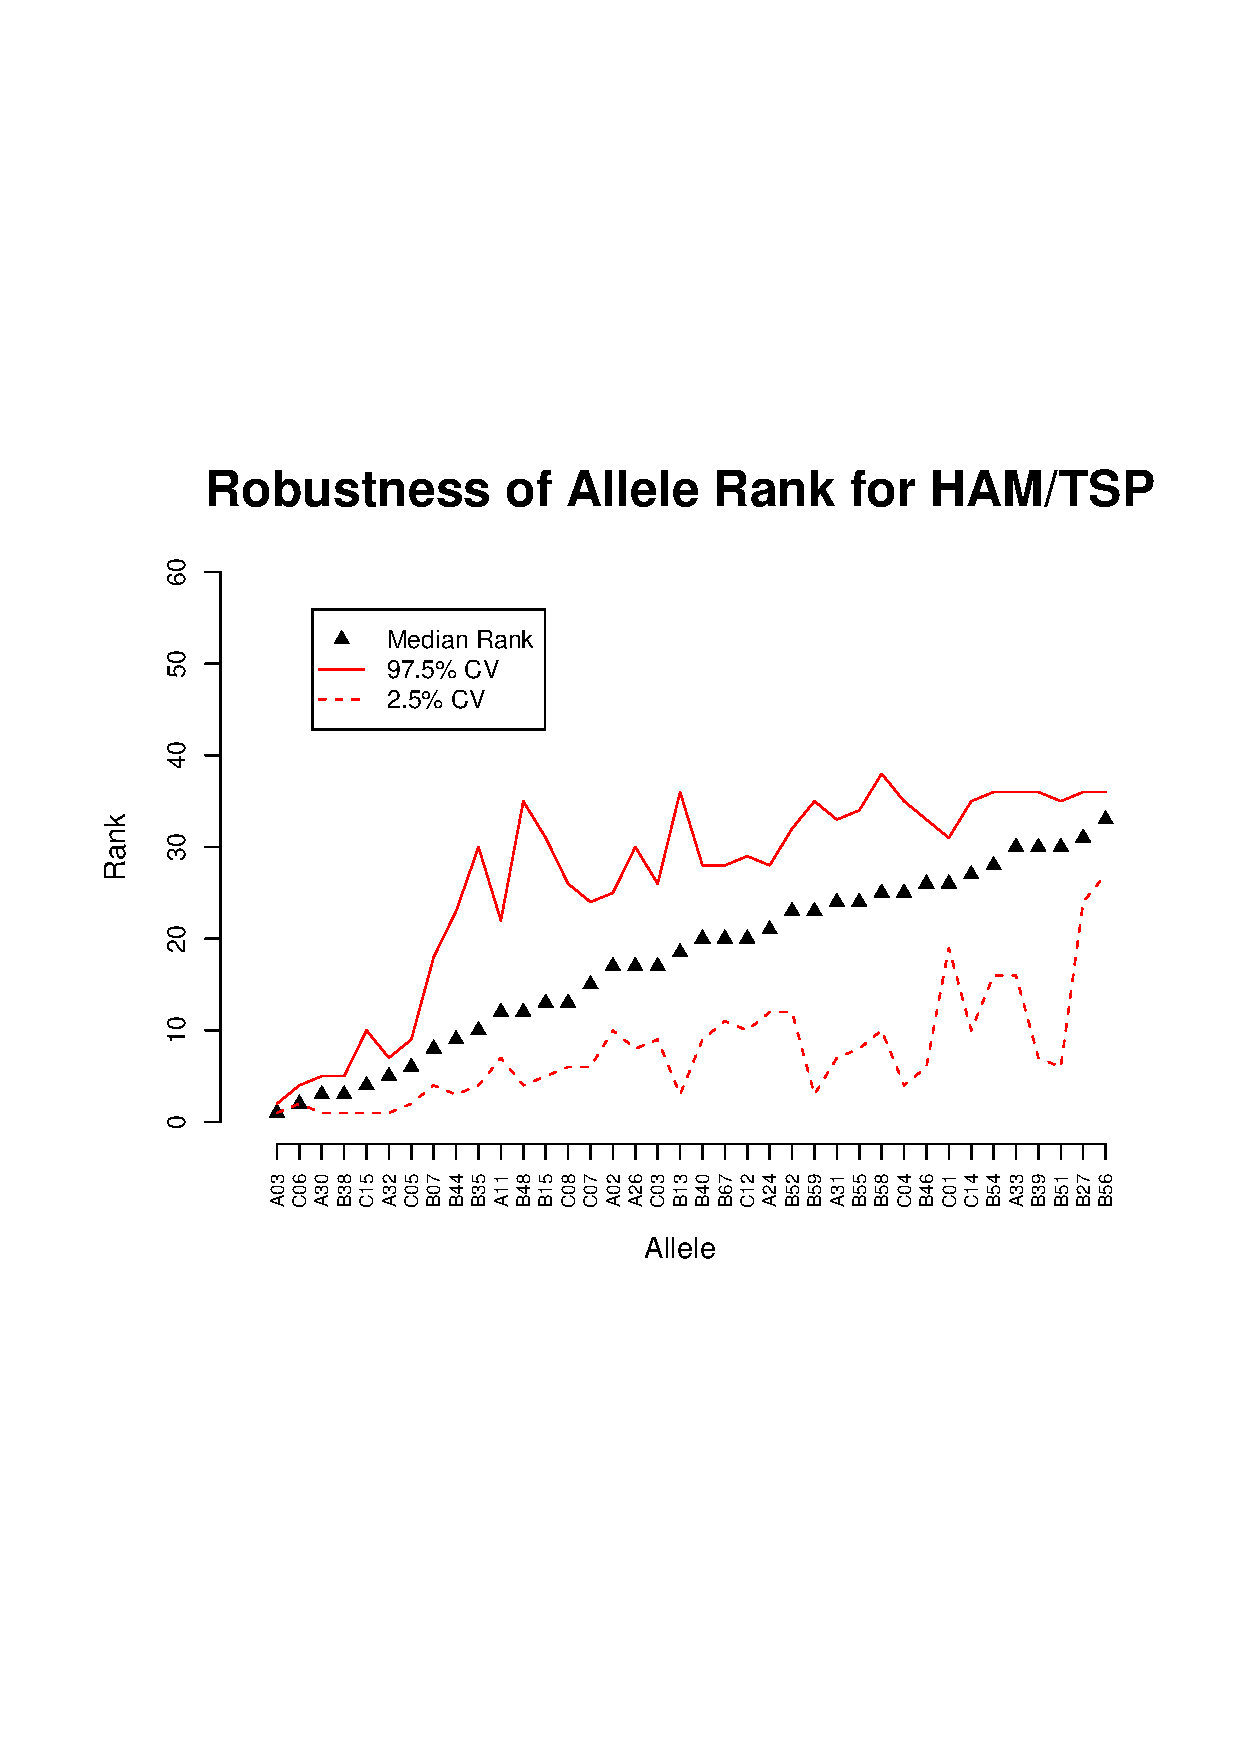
\includegraphics[width=14cm]{./Figures/chapter3/figureRobustHAM}
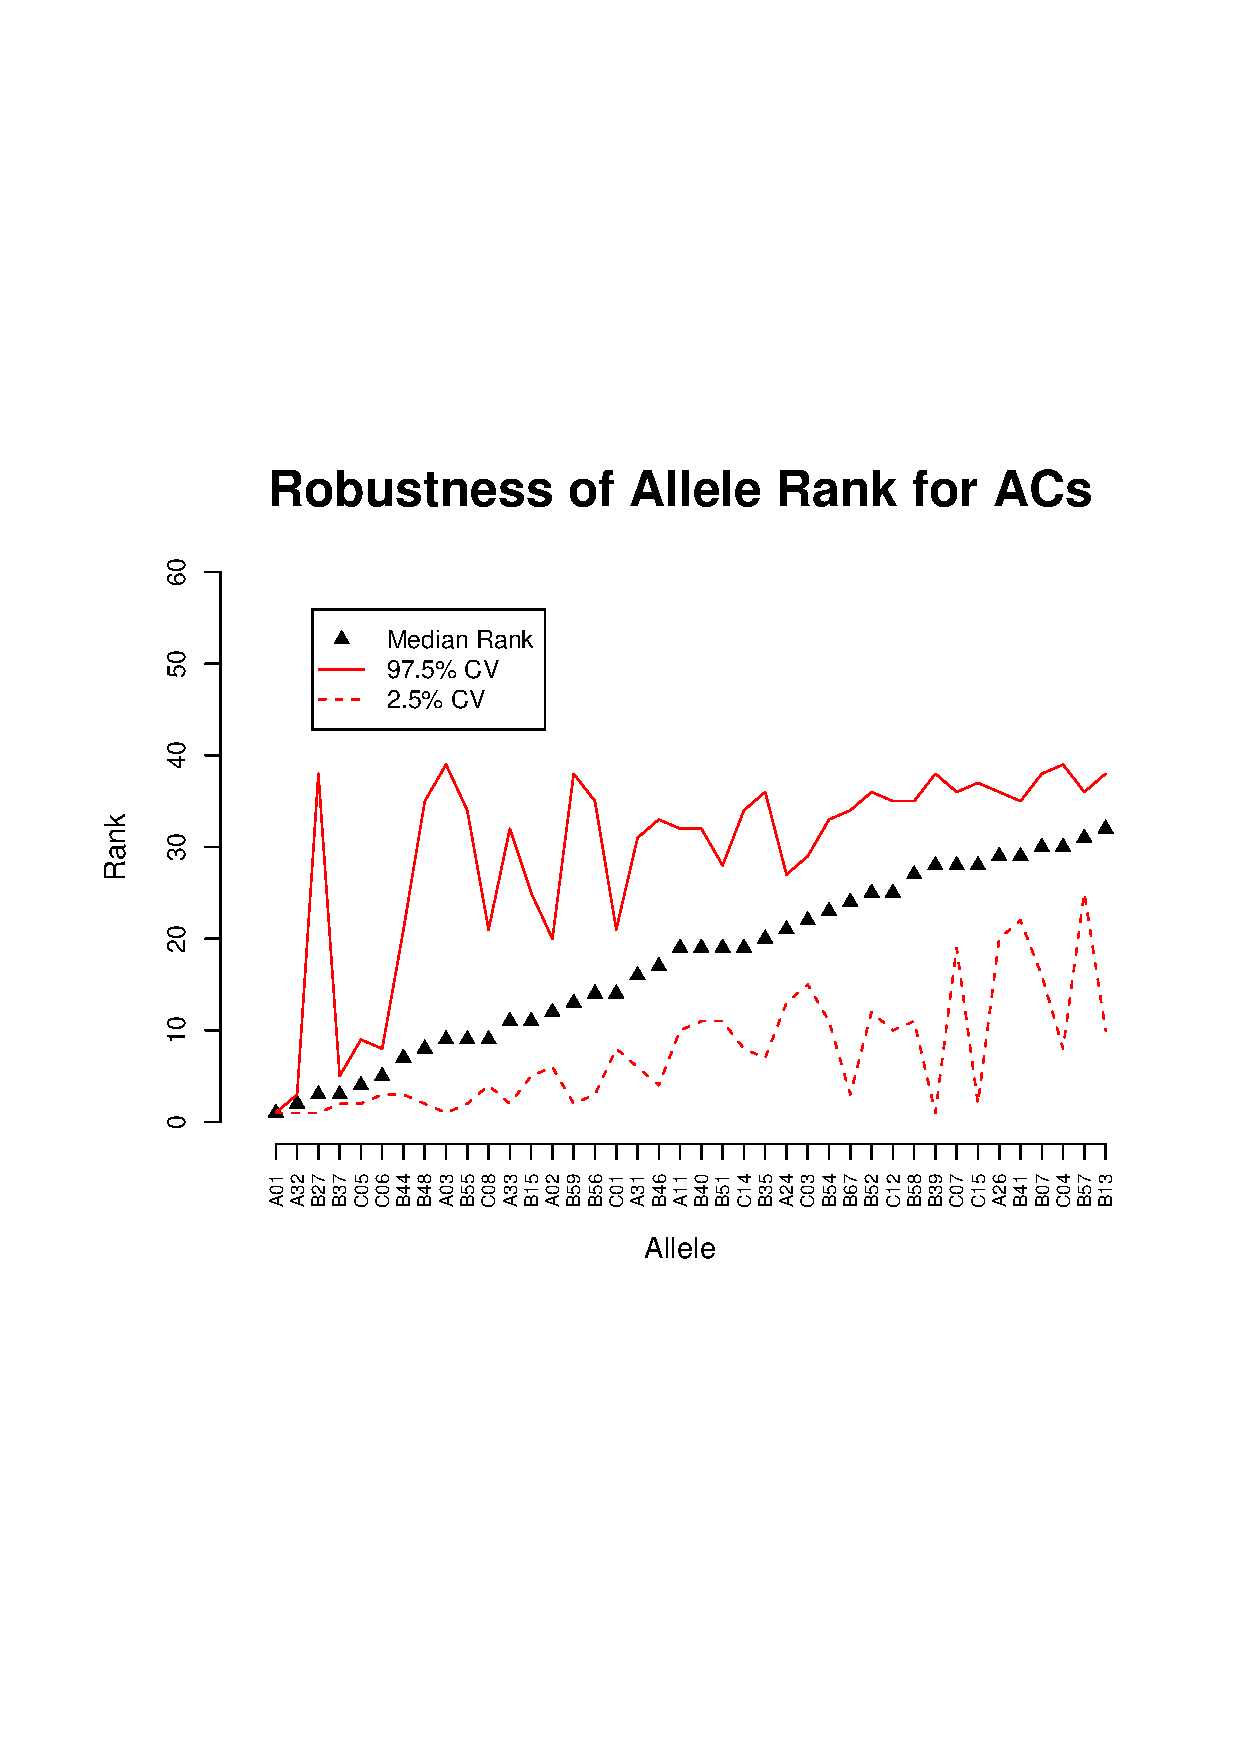
\includegraphics[width=14cm]{./Figures/chapter3/figureRobustAC}
\caption[The robustness of allele ranks]{The allele rankings and robustness, as described in \sref{chapter3/methodsLoad}. Each point gives the allele�s median rank over 2,000 iterations. The area between the solid dot and dotted lines gives the 95\% confidence interval of the value}
\label{chapter3/figureRobust}
\end{figure}

\section{Discussion}\label{chapter3/discussion}

Previous studies have clearly demonstrated the protective effect of \gene{Cw*08} and \gene{A*02} in terms of proviral load in aymptomatic carriers and disease risk \citep{Jeffery1999, Jeffery2000}. This would suggest a protective effect of a strong CTL response. The finding that heterozygosity also resulted in a significantly reduced proviral load suggested the presence of other protective alleles. We reanalysed the Kagoshima Cohort to look for any other allele effects with the goal of assembling the alleles of the cohort into larger sets of protective and detrimental alleles in order to give our epitope analysis greater power. 

\tref{chapter3/tableSummary} gives the summary of results for the tests of association between each allele in the Kagoshima Cohort against disease risk and proviral load. Using this combination of tests, we looked for any alleles that were significantly associated with either detrimental or protective outcomes, excluding those already known. From this analysis, no new alleles could be significantly linked with either disease status or proviral load. There are multiple reasons why this could happen: certain alleles may not have been represented at a high enough frequency in the Kagoshima cohort. More specifically, each individual expresses 6 co-dominant MHC class I alleles, which makes it a statistically difficult task to understand each allele's effect at the individual level. For example, the effect of possessing both detrimental and beneficial alleles may be additive or dominant in either direction. 
%(we specifically explore this question in \aref{AppendixC}, \sref{appendixc/AlleleEffect}).
We decided at this point to proceed with our definition of beneficial and detrimental alleles limited to \gene{Cw*08}/\gene{A*02} and \gene{B*54} respectively. By using epitope prediction software each allele could be clearly defined in terms of their epitope properties - a definition that takes into account funtionality and would be a more nuanced method of separating alleles compared to  their association with disease risk and proviral load. This analysis follows in \cref{Chapter4} and \cref{Chapter6}.